\documentclass[pdftex,12pt]{article}

\usepackage[utf8]{inputenc}
\usepackage[english]{babel}
\usepackage[english]{isodate}
\usepackage[parfill]{parskip}
\usepackage[pdftex]{graphicx}
\usepackage{todonotes} % \todo{note} \listoftodos
\usepackage{microtype}
\usepackage{titling}
\usepackage{booktabs}
\usepackage{multirow}
\usepackage{hyperref}
\usepackage{float}
\usepackage{longtable}
\usepackage{tablefootnote}

% Commands
\newcommand{\HRule}{\rule{\linewidth}{0.5mm}}

\title{Maxwell Katz for Dummies}
\author{Harrison J Katz}
\date{\today}

\begin{document}
\pagenumbering{Roman}

% Title Page
\begin{titlepage}
    \begin{center}
        \ % starts a paragraph so tex is happy
        \textsc{\huge \thetitle}\\
        \textsc{An Instruction Manual}\\[1em]
        \HRule \\[1em]

        \begin{figure}[h!]
            \centering
            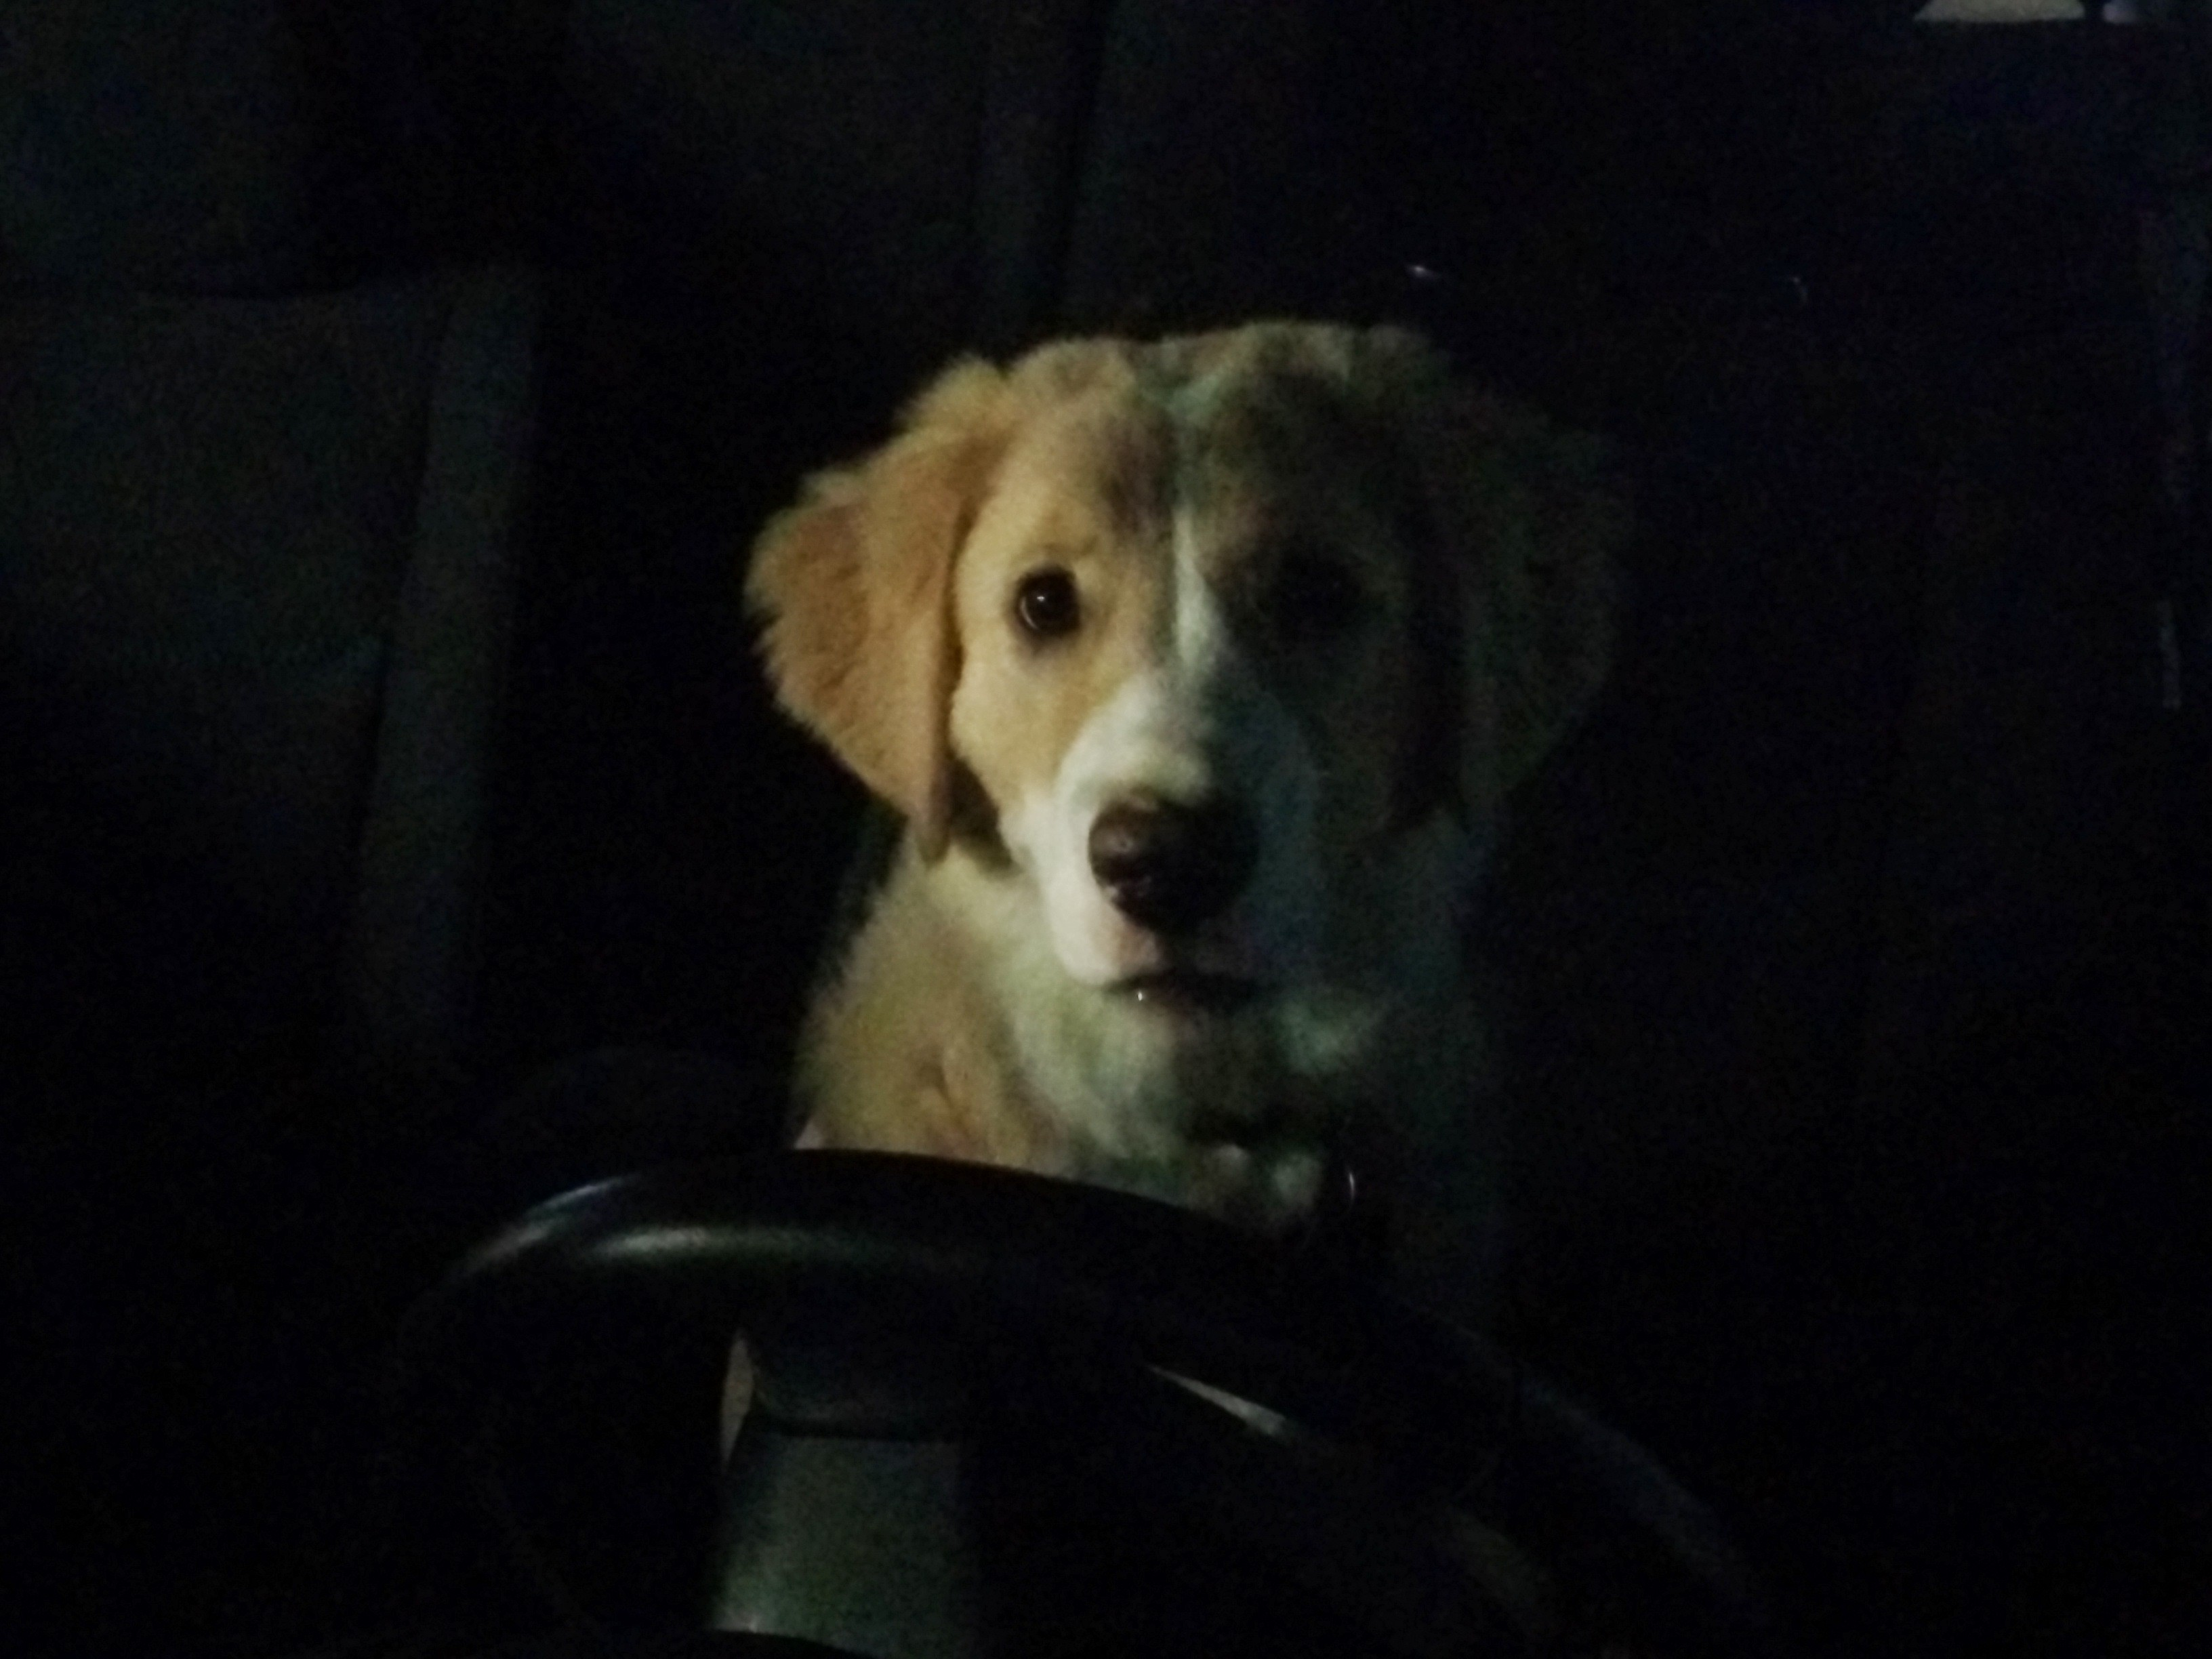
\includegraphics[width=.75\textwidth]{./images/max/title.jpg}
            \caption{Maxwell learning to operate a motor-vehicle.}
            \label{fig:max_title}
        \end{figure}

        % Bottom of the page
        \vfill
        {
            \large \theauthor \  --- \large \thedate
        }

    \end{center}
\end{titlepage}


% Contents
\newpage
\tableofcontents
\todo{Information, emergency, contacts, medicines}
\todo{Schedule, eating, walks, play}
\todo{Training, commands, disciplen, rewards}
\todo{What to do if...}
\todo{Extra information, figures, pictures, etc...}

% Figures
\newpage
\listoffigures

% Document
\newpage
\pagenumbering{arabic}

\section{Introduction}

So, you've been wrangled into babysitting a dog. Not just any dog though, Max.
\emph{Sigh.} What are you going to do? Maxwell Katz (no middle name) is a
rambunctions, destructive, incorrigible goofball, yet he will tug at your
heartstrings with his lovable face and ears. What should you do? What does he
eat? \emph{Oh no!} What does he do for fun? What should I do in the case of
emergency? This may seem like a lot to handle, but fear not, all of this and
more will be answered in this manual.

\newpage
\section{Emergency Information}

\begin{table}[H]
    \begin{longtable}{@{}ll@{}}
        \toprule
        \multicolumn{2}{c}{Pet Information}                                                                              \\ \midrule
        Name          & Maxwell Katz                                                                                     \\
        Answers to    & "Max!" "Maxwell" "*whistle* Come here!"                                                          \\
        Breed         & Golden Retriever / Great Pyrenees                                                                \\
        Color         & Golden White (Toasted Marsh-mellow)                                                              \\
        Date of Birth & January 9th, 2014                                                                                \\
        Health Issues & N/A                                                                                              \\
        Allergies     & Chocolate                                                                                        \\
        Other         & Has 2 extra toes, a trait of Pyrenees                                                            \\ \midrule
        \multicolumn{2}{c}{Owner Information}                                                                            \\ \midrule
        Name          & Harrison John Katz                                                                               \\
        Phone \#      & 706.801.5289                                                                                     \\
        Email         & hjkatz03@gmail.com                                                                               \\ \midrule
        \multicolumn{2}{c}{Emergency Contact}                                                                            \\ \midrule
        Name          & Laura Katz                                                                                       \\
        Relation      & Mother of Harrison Katz                                                                          \\
        Phone \#      & 706.612.4572                                                                                     \\
        Email         & ldkatz38@gmail.com                                                                               \\ \midrule
        \multicolumn{2}{c}{Veterinary Information}                                                                       \\ \midrule
        Name          & Peachtree Hills Animal Hospital                                                                  \\
        Phone \#      & 404.812.9880                                                                                     \\
        Address       & \multirow{3}{*}{\begin{tabular}[c]{@{}l@{}}3106 Early Street\\ Atlanta, GA\\ 30305\end{tabular}} \\
                      &                                                                                                  \\
                      &                                                                                                  \\
        Website       & \url{http://www.peachtreehillsvet.com}                                                           \\
        Email         & info@peachtreehillsvet.com                                                                       \\
        Hours         & Monday-Friday, 8am-6pm                                                                           \\
        Emergency     & \url{http://www.peachtreehillsvet.com/emergencies}                                            
    \end{longtable}
    \label{tab:information}
\end{table}

\newpage
\section{Schedule}

Maxwell's schedule is extremely rigourous, and must be kept with the up most
scrutiny. He requires attention literally 24 hours a day, 7 days a week, and
without this given to him, I fear he may become deprived, depressed, or
worse...dead. Below is his main schedule for a normal week, keep in mind that
Maxwell is crate trained. His crate is a safe zone, a home away from home. Feel
free to place Max in his crate whenever he becomes too much of a hazard.

\begin{table}[h]
    \caption{Maxwell's rigorous daily schedule.}
    \begin{longtable}{r|ll}
                        & Weekday               & Weekend               \\ \hline \\
        Midnight - 7 am & Sleeping              & Sleeping              \\
        8 am            & Morning Walk (E,O)
                          \tablefootnote{Pee and Poop}
                                                & Morning Walk (E,O)    \\
        9 am            & Breakfast             & Breakfast             \\
        10 am           & Sleeping              & Play Time             \\
        11 am           & Sleeping              & Play Time             \\
        Noon            & Sleeping              & Afternoon Walk (E)
                                                  \tablefootnote{Pee only}
                                                                        \\
        1 pm            & Sleeping              & Play Time             \\
        2 pm            & Sleeping              & Park Time             \\
        3 pm            & Sleeping              & Nap Time              \\
        4 pm            & Sleeping              & Nap Time              \\
        5 pm            & Evening Walk (E)      & Evening Walk (E)      \\
        6 pm            & Dinner                & Dinner                \\
        7 pm            & After Dinner Walk (O)
                          \tablefootnote{Poop only}
                                                & After Dinner Walk (O) \\
        8 pm            & Play Time             & Play Time             \\
        9 pm            & Play Time             & Play Time             \\
        10 pm           & Night Walk (E)        & Night Walk (E)        \\
        11 pm           & Sleeping              & Sleeping              \\
    \end{longtable}
    \label{tab:schedule}
\end{table}

\pagebreak

As you should be able to tell by now, this is a sarcastic document. I hope that
you read the whole file, although all the basic information will be presented in
tables and lists. Below you will find a descriptive list of Max's rituals.
\\

\begin{itemize}\label{itm:schedule}
    \item \textbf{Sleeping:} Max's sleeping schedule is pretty lax. He sleeps 
        quite often, and is adorable the entire time. Keep in mind the following:
        \begin{itemize}
            \item Crating Max for sleep time is OK
            \item Max can be petted while he is asleep
            \item Max sheds, so be aware of letting him on the bed
        \end{itemize}
    \item \textbf{Walks:} Walking Max is a fun adventure. He is learning that he
        is strong, and WILL PULL. He has a special leash that can be used if he 
        gets out of hand. See \todo{add reference for special harness}.
        \begin{itemize}
            \item Walks can be as short as 30 secs, or as long as 30 mins
            \item Some walks are pee, some poop, some both
                  (See Table~\ref{tab:schedule} on page~\pageref{tab:schedule})
            \item Maxwell is trained to go to the bathroom on command
                  (See \todo{insert reference to commands})
        \end{itemize}
    \item \textbf{Feeding:} Maxwell eats twice a day, once in the morning and
        once in the evening. He also receives water during each meal.
        \begin{itemize}
            \item Each meal consists of 1.5 cups of dog food
            \item Max is trained to wait til eating
                  (See \todo{insert reference to commands})
            \item Max eats fast, and he must be walked immediatly after dinner
        \end{itemize}
    \item \textbf{Play Time:} Max loves to play! He plays ball, tug of war, chew
        the shoes, eat the garbage, and lots more\ldots!
        \begin{itemize}
            \item Max comes with a plethera of toys
                  (See \todo{insert reference to Max items})
            \item Max is very energetic, you have been warned
        \end{itemize}
\end{itemize}

% Todos
\newpage
\listoftodos

\end{document}
